%\documentclass[draft]{llncs}
\documentclass{llncs}

\usepackage[utf8]{inputenc}
\usepackage{makeidx}
\usepackage{booktabs}
\usepackage{llncsdoc}
\usepackage[pdftex]{graphicx}
\usepackage{listings}
%\lstset{ %
%language=Octave,                % choose the language of the code
%basicstyle=\footnotesize,       % the size of the fonts that are used for the code
%numbers=left,                   % where to put the line-numbers
%numberstyle=\footnotesize,      % the size of the fonts that are used for the line-numbers
%stepnumber=2,                   % the step between two line-numbers. If it's 1 each line will be numbered
%numbersep=5pt,                  % how far the line-numbers are from the code
%backgroundcolor=\color{white},  % choose the background color. You must add \usepackage{color}
%showspaces=false,               % show spaces adding particular underscores
%showstringspaces=false,         % underline spaces within strings
%showtabs=false,                 % show tabs within strings adding particular underscores
%frame=single,	                % adds a frame around the code
%tabsize=2,	                % sets default tabsize to 2 spaces
%captionpos=b,                   % sets the caption-position to bottom
%breaklines=true,                % sets automatic line breaking
%breakatwhitespace=false,        % sets if automatic breaks should only happen at whitespace
%title=\lstname,                 % show the filename of files included with \lstinputlisting; also try caption instead of title
%escapeinside={\%*}{*)}          % if you want to add a comment within your code
%}

\usepackage{url}
\usepackage{fancyvrb}
\usepackage{capt-of}
\usepackage[plainpages=false,pdfpagelabels]{hyperref}
\usepackage{amsmath}
\usepackage[margin=10pt,font=small,labelfont=bf,justification=centerlast]{caption}

% english bibliography
\usepackage[english]{babel}
\usepackage{babelbib}

\makeatletter
\AtBeginDocument{%
  \renewcommand*{\thelstlisting}{\arabic{lstlisting}}%
  }
\makeatother

\title{CATpiler}
\subtitle{A Compiler for the LOLCODE language}
\author{Stephanie Stroka}
\institute{\email{stephanie.stroka@sbg.ac.at} \\ Department of Applied Informatics \\University of Salzburg}
\date{\today}
\begin{document}

\maketitle

\abstract{This document describes the design and functionality of CATpiler - a compiler for the LOLCODE\footnote{\url{http://www.lolcode.com}} language. In the following, I would like to give an overview over the input language characteristics, the lexical analysis and the parsing process, as well as the semantic analysis, code generation and memory management done by CATpiler. The project has been realized during the Compiler Construction course lead by Prof. Christoph Kirsch (2010).}

%%%%%%%%%%%%%%%%%%%%%%%%%%%%%%%%%%%%%%%%%%%%%%%%%%%%
%%%%%%%%%%%%%%%%%%%% SECTION %%%%%%%%%%%%%%%%%%%%%%%
%%%%%%%%%%%%%%%%%%%%%%%%%%%%%%%%%%%%%%%%%%%%%%%%%%%%
\section{Language Description}

LOLCODE can be categorized as an esoteric programming language, which is under construction since May 2007. The main characteristics are the non-classic way of appointing keywords, which will be discussed later, prefix instead of infix operators and the optional type definition. 

The current specification 1.2 does not define array and record handling, and does also not allow to use single characters instead of strings. Thus, to fulfill the classes` requirements, the syntax specification has been slightly adapted.

%%%%%%%%%%%%%%%%%%%% SUBSECTION %%%%%%%%%%%%%%%%%%%%%%%
\subsection{Syntax}

The notion of \textit{non-classic way of appointing keywords} gets clear if we have a look at the language comparision between (pseudo) C and LOLCODE syntax, shown in Listing \ref{tab:syntax}. As one can see, keywords can contain blank characters, or in other words, a keyword may consist of several words. 

\begin{table}[h]\scriptsize
\begin{center}
	\begin{tabular}{ll}
\toprule
\textbf{C-alike syntax} & \textbf{LOLCode syntax} \\
\midrule
$//$ & BTW \\
$/* ... */$&OBTW ... TLDR \\
$\#include <module.h>$&CAN HAS module \\
$main()$&HAI \\
$exit()$&KTHXBYE \\
$<type> <var>$&I HAS A $<var>$ \\
$... $&$<var>$ IS NOW A $<type>$ \\
$<var> = <value>$&$<var>$ R $<value>$ \\
$char$&CHAR \\
$char[\ ]$&CHARZ \\
$int$&NUMBR \\
$int[\ ]$&NUMBRZ \\
$boolean$&TROOF \\
$boolean[\ ]$&TROOFZ \\
$i[4]$&i.4 \\
$someStruct.element$&someStruct$->$element \\
$untyped$&NOOB \\
$true $& WIN \\
$false $& FAIL \\
$\setminus n$&:) \\
$"$&:" \\
$<x> + <y>$&SUM OF $<x>$ AN $<y>$ \\
$<x> - <y>$&DIFF OF $<x>$ AN $<y>$ \\
$<x> * <y>$&PRODUKT OF $<x>$ AN $<y>$ \\
$<x> / <y>$&QUOSHUNT OF $<x>$ AN $<y>$ \\
$max(<x>,<y>)$&BIGGR OF $<x>$ AN $<y>$ \\
$min(<x>,<y>)$&SMALLR OF $<x>$ AN $<y>$ \\

$ <x> \&\& <y> $ & BOTH OF $<x>$ AN $<y> $ \\
$ <x> || <y> $& EITHER OF $<x>$ AN $<y> $ \\
$ !<x> $& NOT $<x>$ \\

$ <x_{1}> \&\& <x_{2}> \&\& ... \&\& <x_{i}> $& ALL OF $<x_{1}>$ AN $<x_{2}>$ AN ... AN $<x_{i}>$ MKAY \\
$ <x_{1}> || <x_{2}> || ... || <x_{i}> $& ANY OF $<x_{1}>$ AN $<x_{2}>$ AN ... AN $<x_{i}>$ MKAY \\

$ <x> == <y> $& BOTH SAEM $<x>$ AN $<y> $ \\
$ <x> != <y> $& DIFFRINT $<x>$ AN $<y> $ \\
$ <x> >= <y> $& BOTH SAEM $<x>$ AN BIGGR OF $<x>$ AN $<y> $ \\
$ <x> <= <y> $& BOTH SAEM $<x>$ AN SMALLR OF $<x>$ AN $<y> $ \\

$ <x> > <y> $& DIFFRINT $<x>$ AN BIGGR OF $<x>$ AN $<y>$ \\
$ <x> < <y> $& DIFFRINT $<x>$ AN SMALLR OF $<x>$ AN $<y>$ \\

%$ cast $&$ MAEK <expr> A <type>$ \\
% &$ <var> R MAEK <var> A <type>$ \\

%$ print() $&$ VISIBLE $ \\
%$to string$&$:<var>$ \\
%$ get() $&$ GIMMEH $ \\

$ if $& ORLY? \\
$ then $& YA RLY \\
$ else if $& MEBBE \\
$ else $& NO WAI \\
$ end-of-if $& OIC \\

$ loop $& IM IN YR $<label>$ YR $<var>$ [TIL|WILE $<expr>$] \\
$ loop-end $& IM OUTTA YR $<label> $ \\

$ function\_label(<arg1>,arg2>...) $& CAN U $<function\_label>$ [YR $<arg1>$ AN YR $<arg2>$ ...] \\
$ void\ function\_label(<arg1>,arg2>...) \{ $& HOW DUZ I $<function\_label>$ [YR $<arg1>$ AN YR $<arg2>$ ...] \\
$ \}\ (function-end) $& IF YOU SAY SO \\

$ struct <label> $& STUFF $<label>$ \\
$ struct-end $& THATSIT \\

$ malloc() $& DOWANT \\

\bottomrule
	\end{tabular}
	\captionof{table}{Sytax accepted by CATpiler}
	\label{tab:syntax}
\end{center}
\end{table}

There are two ways of dealing with multiple-word keywords regarding lexical analysis. The first is that we search for the whole keyword, e.g. \textit{"HOW DUZ I"}, which has the advantage of eliminating ambiguous keyword-tokens like \textit{"I"}. The second one is to scan for each single keyword token, e.g. \textit{"HOW"}, \textit{"DUZ"} and \textit{"I"}, respectively, and leave the "real" keyword determination to the parsing process. The benefit that we get by choosing the second approach is to be able to better deal with literal errors and skipped keyword-tokens. I chose the second approach, which results in checking source code tokens against 73 diverse keyword tokens. 
Thus, the lexical syntax analysis is the process of checking source code words against 73 deterministic finite automatons (DFA) plus three more DFAs for character strings, integers and identifiers. 

Token scanning is a depth-first search. We, therefore, go through the list of tokens and check the first character of the input string against the first character of the token string. Non-equal characters result in a remove of the token and the checking of the next token. If we found a token that matches the first character, we return it as a candidate token and check the remaining characters. For keywords, which start with equal characters, we may need to revert our choice of the candidate token and chose another one. It may also happen that a source code token starts with the same sequence as keyword token, but exceed the string length and are therefore recognized as identifiers. 


%%%%%%%%%%%%%%%%%%%% SUBSECTION %%%%%%%%%%%%%%%%%%%%%%%
\subsection{Parsing}

\begin{table}[h]\scriptsize
\begin{center}
	\begin{tabular}{ll}

\toprule
\textbf{Non-Terminal} & \textbf{Production} \\
\midrule
$<$LETTER$>$ & $::=$ "a" $|$ ... $|$ "z" $|$ "A" $|$ ... $|$ "Z" . \\
$<$DIGIT\_NO\_ZERO$>$ & $::=$ "1" $|$ "2" $|$ "3" $|$ "4" $|$ "5" $|$ "6" $|$ "7" $|$ "8" $|$ "9" . \\
$<$DIGIT$>$ & $::=$ "0" $|$ $<$DIGIT\_NO\_ZERO$>$ . \\
$<$NUM$>$ & $::=$ $<$DIGIT\_NO\_ZERO$>$ $\lbrace$ $<$DIGIT$>$ $\rbrace$ . \\
$<$UNDERSCORE$>$ & $::=$ "\_" . \\
$<$SPECIAL\_CHAR$>$ & $ ::= "\ " | <$UNDERSCORE$>$ $|$ $<$CTRL\_CHAR$> | "-" | "." | "," | ";" | "::" | ":)" | $ \\ 
			& \qquad $ "!" | ":"" | "\$" | "\%" | "\&" | "/" | "(" | ")" | "=" | "?" | "\setminus" | "'" | "*" | "+" | ">" | "<" . $ \\
$<$STRING$>$ & $ ::= """ ( \lbrace <$LETTER$>$ $|$ $<$DIGIT$>$ $|$ $<$SPECIAL\_CHAR$>$ $\rbrace$) """ . \\
$<$BOOL$>$ & $::=$ "WIN" $|$ "FAIL" . \\
$<$IDENTIFIER$>$ & $::=$ $<$LETTER$>$ $\lbrace$ $<$LETTER$>$ $|$ $<$DIGIT$>$ $|$ $<$UNDERSCORE$>$ $\rbrace$ . \\
$<$TYPE$>$ & $::=$ "TROOF" $|$ "NUMBR" $|$ "CHAR" . \\
		& \qquad "TROOFZ" $|$ "NUMBRZ" $|$ "CHARZ" . \\
$<$GEN\_EXPR$>$ & $::=$ ("BOTH SAEM" $|$ "DIFFRINT") $<$OPERATION$>$ "AN" $<$OPERATION$>$ . \\
$<$INF\_EXPR$>$ & $::=$ ("ALL OF" $|$ "ANY OF") $<$BOOL\_OP$>$ "AN" $<$BOOL\_OP$>$ \\
 & $::=$ $\lbrace$ "AN" $<$BOOL\_OP$>$ $\rbrace$ "MKAY" . \\
$<$BI\_EXPR$>$ & $::=$ $<$BOOL\_OP$>$  $|$ $<$GEN\_EXPR$>$ . \\
$<$EXPR$>$ & $::=$ $<$BI\_EXPR$>$ $|$ $<$INF\_EXPR$>$ $|$ ($<$BOOL$>$$|$ $<$IDENTIFIER$>$) . \\
%$<$IO\_OP$>$ & $::=$ VISIBLE $<$VALUE$>$ $|$ GIMMEH $<$IDENTIFIER$>$ . \\
$<$BOOL\_OP$>$ & $::=$ (("BOTH OF" $|$ "EITHER OF") $<$EXPR$>$ "AN" $<$EXPR$>$) $|$ \\ 
		& \qquad("NOT" $<$EXPR$>$) . \\
$<$STR\_OP$>$ & $::=$ $<$STRING$>$ $|$ $<$IDENTIFIER$>$ . \\ 
$<$NUM\_OP$>$ & $ ::=$ ("SUM OF" $|$ "DIFF OF" $|$ "PRODUKT OF" $|$ "QUOSHUNT OF" $|$ \\ 
		& \qquad "BIGGR OF" $|$ "SMALLR OF") $<$NUM\_OP$>$ "AN" $<$NUM\_OP$>$ $|$ \\
		& \qquad ($<$NUM$>$ $|$ $<$IDENTIFIER$>$) . \\
$<$OPERATION$>$ & $ ::=$ $<$NUM\_OP$>$ $|$ $<$BOOL\_OP$>$ $|$ $<$STR\_OP$>$ . \\
$<$VAR\_INIT$>$ & $::=$ "I HAS A" $<$IDENTIFIER$>$ . \\
$<$VAR\_DECL$>$ & $::=$ $<$IDENTIFIER$>$ "IS NOW A" $<$TYPE$>$ . \\
$<$VAR\_ASSIGN$>$ & $::=$ $<$IDENTIFIER$>$ "R" $<$OPERATION$>$ . \\
$<$IF$>$ & $::=$ $<$EXPR$>$ ORLY? YA RLY $\lbrace$ $<$STATEMENT$>$ $\rbrace$ \\ 
		& \qquad $\lbrace$ MEBBE $<$EXPR$>$ $\lbrace$ $<$STATEMENT$>$ $\rbrace$ $\rbrace$ \\
		& \qquad $[$ NO WAI $\lbrace$ $<$STATEMENT$>$ $\rbrace$ $]$ $\rbrace$ OIC . \\
$<$LOOP$>$ & $ ::=$ "IM IN YR" $<$IDENTIFIER$>$ $[$YR $<$IDENTIFIER$>$ $]$ $[$WILE$|$TIL $<$EXPR$>$ $]$ \\ 
		& \qquad $\lbrace$ $<$STATEMENT$>$ $\rbrace$ "IM OUTTA YR" $<$IDENTIFIER$>$ . \\
$<$FLOW\_CONTROL$>$ & $ ::=$ $<$IF$>$ $|$ $<$LOOP$>$ . \\
$<$FUNC\_CALL$>$ & $ ::=$ $<$IDENTIFIER$>$ $\lbrace$ $<$EXPR$>$ $\rbrace$ . \\
$<$STATEMENT$>$ & $ ::=$ $<$VAR\_INIT$>$ $|$ $<$VAR\_DECL$>$ $|$ $<$VAR\_ASSIGN$>$ $|$ $<$OPERATION$>$ $|$ \\
		& \qquad $<$FLOW\_CONTROL$>$ $|$ $<$FUNC\_CALL$>$ . \\
$<$FUNCTION$>$ & $ ::=$ "HOW DUZ I" $<$IDENTIFIER$>$ \\ 
		& \qquad $[$YR $<$IDENTIFIER$>$ $\lbrace$AN YR $<$IDENTIFIER$>$ $\rbrace$ $]$ \\ 
		& \qquad $\lbrace$ $<$STATEMENT$>$ $\rbrace$ $\lbrace$ "FOUND YR" $<$EXPR$>$ $|$ "GTFO"$\rbrace$ \\
		& \qquad "IF YOU SAY SO" . \\
$<$MODULE$>$ & $::=$ "CAN HAS" $<$IDENTIFIER$>$ "?" . \\
$<$STRUCT$>$ & $::=$ "STUFF" $\lbrace$ $<$VAR\_INIT$>$ "THATSIT" . \\
$<$MAIN$>$ & $::=$ "HAI" $\lbrace$ $<$STATEMENT$>$ $\rbrace$ "KTHXBYE" . \\
$<$PROGRAMM$>$ & $::=$ $\lbrace$ $<$MODULE$>$ $\rbrace$ $\lbrace$ $<$STRUCT$>$ $\rbrace$ $[$ $<$MAIN$>$ $]$ $\lbrace$ $<$FUNCTION$>$ $\rbrace$ . \\

\bottomrule
	\end{tabular}
	\captionof{table}{Extended Backus-Naur-Form for LOLCODE}
	\label{tab:ebnf}
\end{center}
\end{table}

CATpiler uses a recursive-decent parser to validate the input source against its desired structure, defined in the Extended Backus-Naur Form (EBNF) (see Table \ref{tab:ebnf}). Each non-terminal is represented as a recursive function. To advance the speed of the parsing process, the Scanner assigns a numerical id for each found token, which is than compared in the parser functions. Some of those ids have an important characteristic, which is especially important if they are alternative tokens in an EBNF production. The ids for the keywords \textit{"NUMBR"}, \textit{"CHAR"}, \textit{"TROOF"}, \textit{"NUMBRZ"}, \textit{"CHARZ"}, \textit{"TROOFZ"}, \textit{"SUM"}, \textit{"PRODUKT"}, \textit{"QUOSHUNT"}, \textit{"BIGGR"}, \textit{"SMALLR"} and \textit{"DIFF"} are listed in Table \ref{tab:identifier} in binary form. EBNF alternative keywords share a common group ID.
%EBNF alternatives are grouped together by an and-operation on the keyword ids with a group-id. 

The code-optimization trick is similar to the one proposed in \cite{wirth}. Instead of comparing decimal integer ids by their range (e.g. \textit{"NUMBR"} could have the id 1, \textit{"TROOF"} the id 2 and \textit{"CHAR"} the id 3, so that we would check whether an id is in between the range(1,3)), a logical AND operation is provoked on the keyword id and the check id. The result of the AND operation is either 0, if the keyword does not belong to the group, or the group id respectively.

Identifiers for the other keywords than those listed in Table \ref{tab:identifier} need to be assigned in a way such that a logical AND operation on the id with the check id does not return any of the group ids. To easily guarantee this behavior, we only assign ids that are bigger than $2^4$, or in other words that do not set any bits in the last 4 bits of a word. The remaining $2^{28}$ bits are more than sufficient to be used as identifiers for other keywords.

\begin{table}[h]\scriptsize
\begin{center}
	\begin{tabular}{lccc}

\toprule
\textbf{Keyword} & \textbf{\ Assigned Id\ } & \textbf{\ Group Id\ } & \textbf{\ Check Id\ } \\
\midrule
NUMBR & $\ 0000\ 0000\ 0000\ 0001\ $ & $\ 0000\ 0000\ 0000\ 0001\ $ & $\ 1111\ 1111\ 1111\ 1001\ $ \\
CHAR & $\ 0000\ 0000\ 0000\ 0011\ $ & $\ 0000\ 0000\ 0000\ 0001\ $ & $\ 1111\ 1111\ 1111\ 1001\ $ \\
TROOF & $\ 0000\ 0000\ 0000\ 0101\ $ & $\ 0000\ 0000\ 0000\ 0001\ $ & $\ 1111\ 1111\ 1111\ 1001\ $ \\
\midrule
NUMBRZ & $\ 0000\ 0000\ 0000\ 0010\ $ & $\ 0000\ 0000\ 0000\ 0010\ $ & $\ 1111\ 1111\ 1111\ 0011\ $ \\
CHARZ & $\ 0000\ 0000\ 0000\ 0110\ $ & $\ 0000\ 0000\ 0000\ 0010\ $ & $\ 1111\ 1111\ 1111\ 0011\ $ \\
TROOFZ & $\ 0000\ 0000\ 0000\ 1010\ $ & $\ 0000\ 0000\ 0000\ 0010\ $ & $\ 1111\ 1111\ 1111\ 0011\ $ \\
\midrule
SUM & $\ 0000\ 0000\ 0000\ 0100\ $ & $\ 0000\ 0000\ 0000\ 0100\ $ & $\ 1111\ 1111\ 1100\ 0111\ $ \\
PRODUKT & $\ 0000\ 0000\ 0001\ 0100\ $ & $\ 0000\ 0000\ 0000\ 0100\ $ & $\ 1111\ 1111\ 1100\ 0111\ $ \\
QUOSHUNT & $\ 0000\ 0000\ 0010\ 0100\ $ & $\ 0000\ 0000\ 0000\ 0100\ $ & $\ 1111\ 1111\ 1100\ 0111\ $ \\
DIFF & $\ 0000\ 0000\ 0000\ 1100\ $ & $\ 0000\ 0000\ 0000\ 0100\ $ & $\ 1111\ 1111\ 1100\ 0111\ $ \\
BIGGR & $\ 0000\ 0000\ 0001\ 1100\ $ & $\ 0000\ 0000\ 0000\ 0100\ $ & $\ 1111\ 1111\ 1100\ 0111\ $ \\
SMALLR & $\ 0000\ 0000\ 0010\ 1100\ $ & $\ 0000\ 0000\ 0000\ 0100\ $ & $\ 1111\ 1111\ 1100\ 0111\ $ \\
\midrule
DIFF & $\ 0000\ 0000\ 0000\ 1100\ $ & $\ 0000\ 0000\ 0000\ 1100\ $ & $\ 1111\ 1111\ 1100\ 1111\ $ \\
BIGGR & $\ 0000\ 0000\ 0001\ 1100\ $ & $\ 0000\ 0000\ 0000\ 1100\ $ & $\ 1111\ 1111\ 1100\ 1111\ $ \\
SMALLR & $\ 0000\ 0000\ 0010\ 1100\ $ & $\ 0000\ 0000\ 0000\ 1100\ $ & $\ 1111\ 1111\ 1100\ 1111\ $ \\
\bottomrule
	\end{tabular}
	\captionof{table}{Identifier Assignment for EBNF alternative keywords}
	\label{tab:identifier}
\end{center}
\end{table}

%%%%%%%%%%%%%%%%%%%% SUBSECTION %%%%%%%%%%%%%%%%%%%%%%%
\subsection{Attributed Grammar}

During the lexical analysis and the parsing process, the scanned keywords are extended by attributes represented as string values. Storing identifier names, string and integer values is the preliminary work for building a symbol table. The symbol table contains entries for each source scope, therefore preventing that identifiers are used that have not yet been defined, or that identifiers are defined multiple times. A symbol table entry contains information like \texttt{identifier name}, \texttt{attribute}, \texttt{stack address}, \texttt{heap address}, \texttt{register}, \texttt{type} (i.e. \textit{NUMBR}, \textit{CHARZ}, etc.) and \texttt{category} (i.e. \textit{const}, \textit{var}, \textit{reg}, \textit{heap}). 

Another part of attributing source code is the collection of function definitions and function calls. Instead of storing information about called and implemented functions temporarily in the RAM during compilation, as we do with symbol tables, we write that information into the object code file, to enable separate compilation and late function implementation checking by the Linker.


%%%%%%%%%%%%%%%%%%%% SUBSECTION %%%%%%%%%%%%%%%%%%%%%%%
\subsection{Error Handling}

Code generation is just performed, if the source code has not been marked as faulty. On the other hand it is important to continue parsing if an error has been detected, since it is more convenient for the programmer to come to know all his errors in the source code, and not just the first one. 

Error handling is considered difficulty for the LOLCODE language, because multiple-word keywords provide many options to forget keywords or to introduce typing errors. CATpiler handles programmatic errors pragmatically and considers that keyword skipping happens more frequently. Therefore, a lot of lookahead operations, which give information about the next keyword without adjusting the source code pointer, are necessary. If a lookahead returns a keyword that is not expected, we simply check if the next keyword fits again. An improved version, e.g. to adjust the source pointer if the next keyword also does not fit, and therefore to assume that the keyword contains a typing error, remains future work.

If the error extend is to big to detect a certain statement production, we look up source code tokens until we find the next start of a statement, or until we reach the end of the file, flow-control statement or function. Thus, we can also say that statement begin and end keywords are the \textit{strong symbols} of the LOLCODE language.


%%%%%%%%%%%%%%%%%%%%%%%%%%%%%%%%%%%%%%%%%%%%%%%%%%%%
%%%%%%%%%%%%%%%%%%%% SECTION %%%%%%%%%%%%%%%%%%%%%%%
%%%%%%%%%%%%%%%%%%%%%%%%%%%%%%%%%%%%%%%%%%%%%%%%%%%%
\section{Code Generation}

Immediate code generation is part of the parsing process. Every EBNF-production function immeditaley generates code for the output language, therefore enabling compilation in a single source code iteration. 
The following sections present the target language and code optimizations done by CATpiler.


%%%%%%%%%%%%%%%%%%%% SUBSECTION %%%%%%%%%%%%%%%%%%%%%%%
\subsection{Target Language}

Although there exist a variety of interpreters and one compiler for the .NET platform, CATpiler is the first compiler for the MIPS32 architecture. If computes instructions in MIPS assembler, which can be interpreted and run on any MIPS simulator. The code has been tested for the MARS assembler and simulator platform\footnote{\url{http://courses.missouristate.edu/KenVollmar/MARS/}}.

Listing \ref{tab:identifier} gives an overview over the instructions that have been used to generate code. During parsing, every module generates code that is finally stored in a text file with the file-ending \textit{.cat}. These files will later be linked into a single MIPS text file.

\begin{table}[h]\scriptsize
\begin{center}
	\begin{tabular}{llll}

\toprule
\textbf{Instruction} & \textbf{\ Description\ \ } & \textbf{\ Operation\ \ } & \textbf{Syntax\ } \\
\midrule
add & Adds two registers & $\ \$d = \$s + \$t \ \ $ & add \$d \$s \$t \\
addi & Adds immediate value to register & $\ \$d = \$s + i \ \ $ & addi \$d \$s i \\
sub & Subtracts \$t from \$s & $\ \$d = \$s - \$t \ \ $ & sub \$d \$s \$t \\
subi & Subtracts immediate value from register & $\ \$d = \$s - i \ \ $ & subi \$d \$s i \\
mul & Multiplies two registers & $\ \$d = \$s * \$t \ \ $ & mul \$d \$s \$t \\
muli & Multiplies immediate value to register & $\ \$d = \$s * i \ \ $ & muli \$d \$s i \\
div & Divides \$t from \$s & $\ \$d = \$s\ /\ \$t \ \ $ & div \$d \$s \$t \\
divi & Divides immediate value from register & $\ \$d = \$s\ /\ i \ \ $ & divi \$d \$s i \\
and & AND-operation on two registers & $\ \$d = \$s\ \&\&\ \$t \ \ $ & and \$d \$s \$t \\
andi & AND-operation on register and immediate value & $\ \$d = \$s\ \&\&\ i \ \ $ & andi \$d \$s i \\
or & OR-operation on two registers & $\ \$d = \$s\ ||\ \$t \ \ $ & and \$d \$s \$t \\
ori & OR-operation on register and immediate value & $\ \$d = \$s\ ||\ i \ \ $ & andi \$d \$s i \\
slt & Shift left-operation on two registers & $\ \$d = \$s\ ||\ \$t \ \ $ & and \$d \$s \$t \\
lw & Loads word from address & $\ \$d = address \ \ $ & lw \$d a \\
lb & Loads byte from address & $\ \$d = address \ \ $ & lb \$d a \\
sw & Stores word in address & $\ \$d = address \ \ $ & sw \$d a \\
sb & Stores byte in address & $\ \$d = address \ \ $ & sb \$d a \\
slt & If \$s < \$t, set \$d = 1, otherwise \$d = 0 & & slt \$d \$s \$t \\
beq & Branches if both registers are equal & & beq \$s \$t label \\
bne & Branches if both registers are not equal & & bne \$s \$t label \\
bgez & Branches if the register is greater than or equal zero & & bgez \$s label \\
bgtz & Branches if the register is greater than zero & & bgtz \$s label \\
bltz & Branches if the register is less than zero & & bltz \$s label \\
j & Jumps to label & & j label \\
jal & Stores pc in \$ra register and jumps to label & & jal label \\
\bottomrule
	\end{tabular}
	\captionof{table}{MIPS Instructions}
	\label{tab:identifier}
\end{center}
\end{table}

%%%%%%%%%%%%%%%%%%%% SUBSECTION %%%%%%%%%%%%%%%%%%%%%%%
\subsection{Implemented Functionalities}

The following list provides an overview over the implemented functionalities:

\begin{itemize}
	\item Global and local variable initializations: 
	\begin{itemize}
		\item Integer, characters, boolean primitives
		\item Integer, character and boolean arrays
		\item Structures: Only accessible within a module
		\item Automatically created temporary variable \texttt{IT}: Stores the result of the last computation
		\item Lazy type evaluation: A variable is undefined until explicitly given or until a value is assigned
	\end{itemize}
	\item Operations: 
	\begin{itemize}
		\item Numeric operations (addition, subtraction, multiplication, division, max and min)
		\item String compare
		\item Boolean operations (AND, OR, NOT)
		\item General operations (equal, not-equal)
	\end{itemize}
	\item Flow control: 
	\begin{itemize}
		\item Branching (If-Else If-Else)
		\item Loops (Allows until and while conditions)
	\end{itemize}
	\item Functions: 
	\begin{itemize}
		\item With parameter handing
		\item Allow emergency-escape with keyword \textit{"GTFO"}
		\item Allow return parameters
	\end{itemize}
\end{itemize}

%%%%%%%%%%%%%%%%%%%%%%%%%%%%%%%%%%%%%%%%%%%%%%%%%%%%
%%%%%%%%%%%%%%%%%%%% SECTION %%%%%%%%%%%%%%%%%%%%%%%
%%%%%%%%%%%%%%%%%%%%%%%%%%%%%%%%%%%%%%%%%%%%%%%%%%%%
\section{Memory Management}

Memory Management is important to maintain the memory used by a program. In MIPS, we have an address space of 32 bit. Figure \ref{fig:memlayout} shows the overall memory layout, which is very common in most machines. The memory addresses range from 0x00000000 to 0xffffffff, where 0x00000000 - 0x40000000 and 0x7fffffff - 0xffffffff are reserved for the MIPS OS and the remaining memory is divided into four segments.

The text segment is the part of the memory where our code instructions are stored. Above it, one can find the global data segment for static variables. The heap segment begins on top of the data segment and dynamically grows towards the stack segment, which starts at the top most accessible address 0x7fffffff and shrinks towards the heap segment.

\begin{figure}[h]
  \centering
    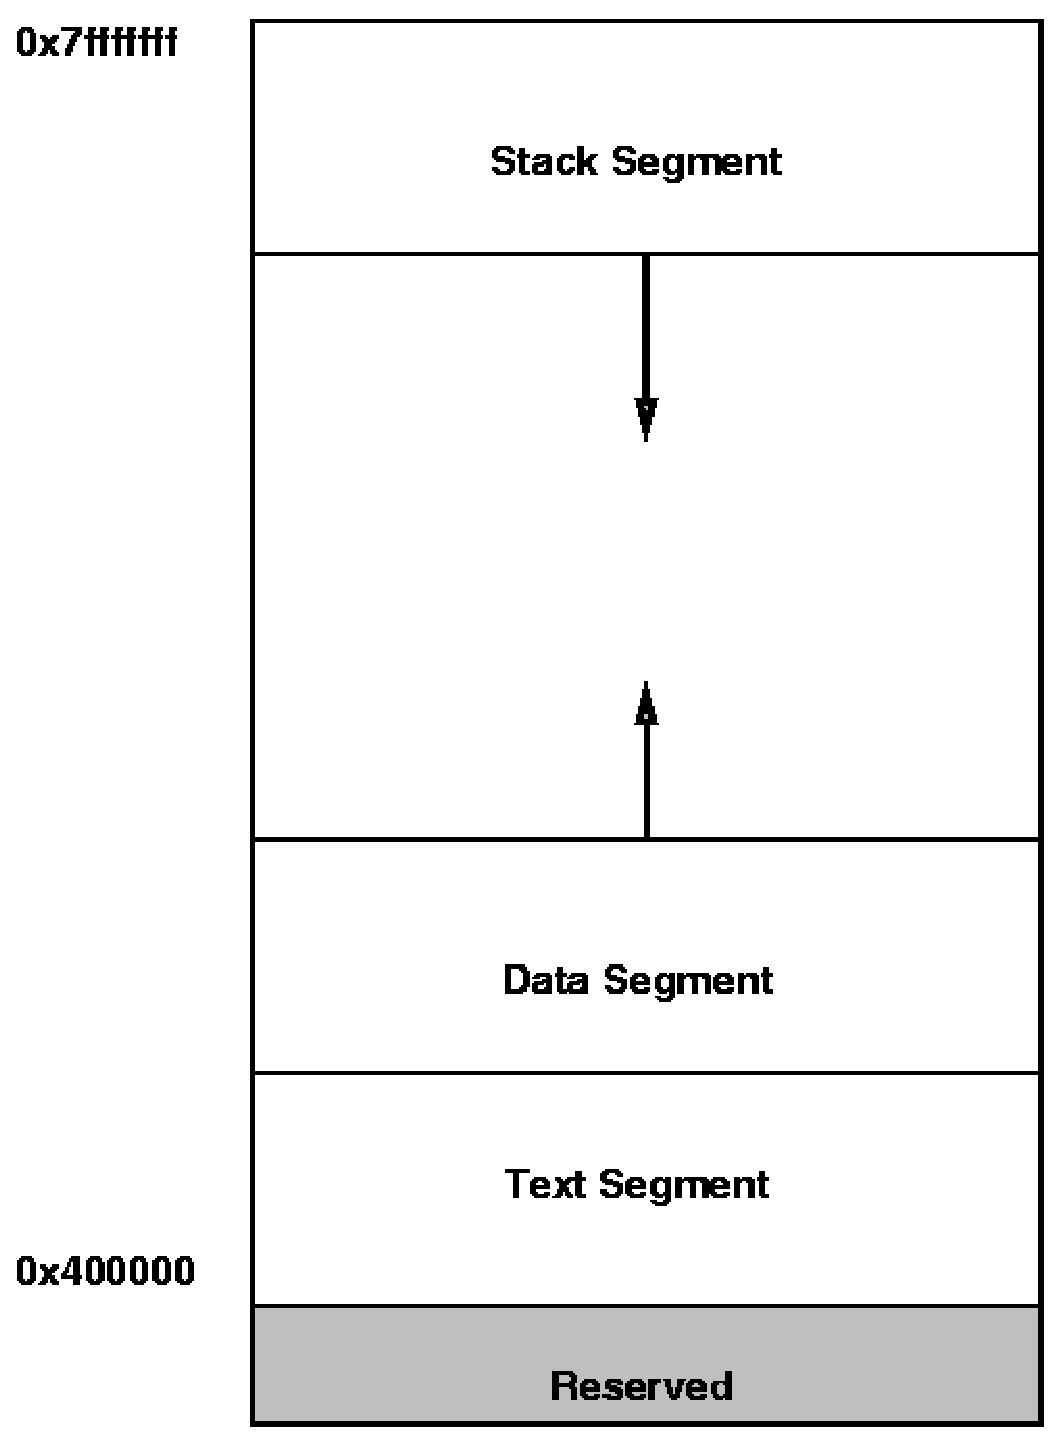
\includegraphics[width=0.5\textwidth]{img/mem_layout}
  \caption{MIPS Memory Layout}
  \label{fig:memlayout}
\end{figure}

Heap management, which is the process of how we allocate and deallocate memory from the heap segment, varies from target code to target code. The SUN JVM (Java Virtual Machine), for example, uses generational garbage collection to allocate and deallocate heap memory dynamically during runtime, whereas in C the programmer usually has to free the allocated memory explicitly. 

Since the CATpiler produces MIPS code which is not intended to run on a (self-designed) virtual machine, the heap must be managed during compile time. To relieve the programmer from freeing memory explicitly, the compiler provides a method to introduce a kind of region based memory management, which is responsible for allocating and reusing memory when an object expires.

The compiler, therefore, divides the heap memory into regions of a fixed size at the beginning of the program. Currently, only 15 heap blocks of size 32 bits are generated (because of compile time performance reasons), which is sufficient for the tests in the test base. Larger programs may require an adjustment of the heap blocks size.

Since we are unaware of the heap block start address during compile time, static heap identifiers, which will be filled with the heap block start addresses later on, are created and stored in the data segment. Listing \ref{lst:heaplabel} shows a fraction of the data and the text segment that is initially constructed by the memory manager. As one can see, heap memory is allocated by a system call (lines 18 - 20), and the region start address is loaded into the address behind the heap label \texttt{hp0} (lines 21 and 22). 

\lstset{language=xml}
\lstinputlisting[
        label=lst:heaplabel,
        captionpos=b,
        caption=Code-Fraction for Memory Partioning,
        numbers=left,
        frame=single,
        breaklines=true,
        basicstyle=\ttfamily\footnotesize,
        keywordstyle=\bfseries,
        commentstyle=\itshape,
        stringstyle=\itshape
]{code/heaplabel.cat}

The memory manager keeps track of which heap blocks will be in use during program execution. This is done by holding a reference map that contains a count for each memory block. Initially, each memory block holds '0' references. When the program comes to a point where an object requests memory, the memory manager assigns one or multiple free heap blocks to the object and sets a reference counter for each heap block to '1'. 

When an object is provided as a function parameter, it's reference count will be increased before the function is called, and decreased after the function return. Hence, we can keep track of the current memory use in each function, and reuse heap blocks if its reference count equals '0' again.

The problem that might be introduced by reference increasing and decreasing is that reference counts for global objects will be set to '0' as soon as we leave the function which assigned memory, even if the object is still expected to be reachable. This may lead to dangling pointers, since the memory could already be reused. An example for that problem is shown in Listing \ref{lst:danglingPointer}.
The solution that CATpiler introduces is to keep the reference count for global variable constantly at '1' by skipping count increase and decrease activities.

\lstset{language=xml}
\lstinputlisting[
        label=lst:danglingPointer,
        captionpos=b,
        caption=Global Variables and the Reference Counting Problem,
        numbers=left,
        frame=single,
        breaklines=true,
        basicstyle=\ttfamily\footnotesize,
        keywordstyle=\bfseries,
        commentstyle=\itshape,
        stringstyle=\itshape
]{code/danglingPointer.lol}

%%%%%%%%%%%%%%%%%%%%%%%%%%%%%%%%%%%%%%%%%%%%%%%%%%%%
%%%%%%%%%%%%%%%%%%%% SECTION %%%%%%%%%%%%%%%%%%%%%%%
%%%%%%%%%%%%%%%%%%%%%%%%%%%%%%%%%%%%%%%%%%%%%%%%%%%%
\section{Separate Compilation}

In large software projects it is often necessary to allow separate compilation in order to speed up the compilation time. A change in one module source file should not necessarily lead to a re-compilation of all other modules. For that reason, the CATpiler only compiles those modules that have not been compiled yet or have been explicitly requested for compilation.

When a file is requested for compilation without any additional parameter, all imported modules will be recursively compiled, too (see Figure \ref{fig:recimport}). Every module will generate an own code file with file ending \textit{.cat}. Each compiled module contains meta-information in the header of the MIPS assembler file. The first line is a timestamp that represents the last modification time, the second line contains all functions that are called from within the module, and the third and last line contains all functions that are defined in this module.

The process of how source files are recursively imported and how code is generated is shown in Figure \ref{fig:recimport} and Figure \ref{fig:link}. The file \textit{module2.lol} is the first module that does not contain any further imports. Thus, it is the first to be compiled. \textit{module4.lol} and \textit{module1.lol} follow subsequently. The \textit{main.lol} has another import on \textit{module2.lol}, but it has already been compiled for the last modification, which can be recognized with the help of the timestamp in the header of \textit{module2.cat}. Therefore it is simply skipped. The next imported module is \textit{module3.lol}, which will be compiled into \textit{module2.cat}. \textit{main.lol} is the last file that is compiled. The handling of cyclic imports remain future work. Currently, one would have to separately compile cyclic modules, which can be done by starting the compiled with the attribute \texttt{"-s"}.

When the compilation process is completed, the Linker copies every \texttt{.cat} file into one single MIPS assembler file with the file ending \textit{.asm}. Header meta-data are copied, too, but will be ignored by the MIPS assembler, since these lines start with a comment character. The instructions and data for heap management will only be copied once.

\begin{figure}[h]
  \centering
    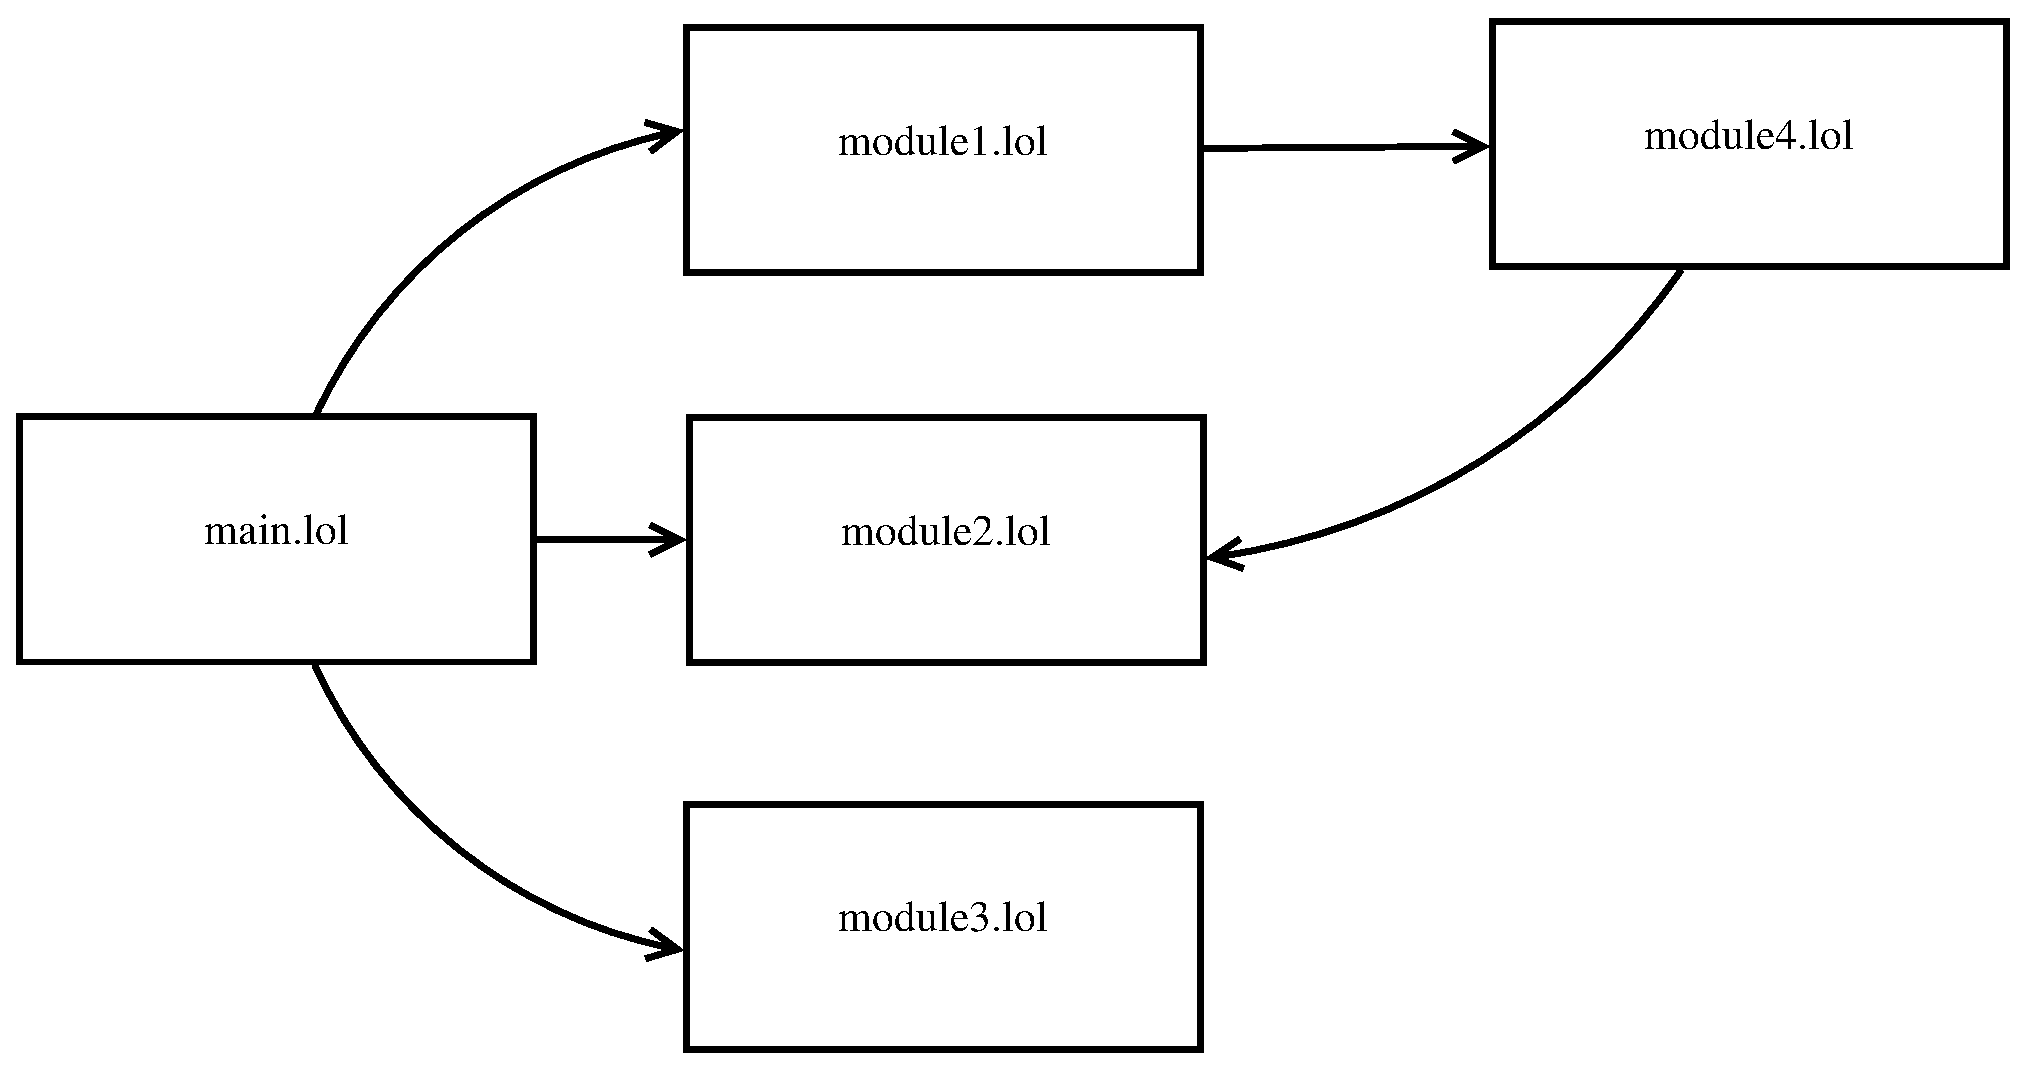
\includegraphics[width=\textwidth]{img/recursive_import}
  \caption{Recursive Import of Module Files}
  \label{fig:recimport}
\end{figure}

\begin{figure}[h]
  \centering
    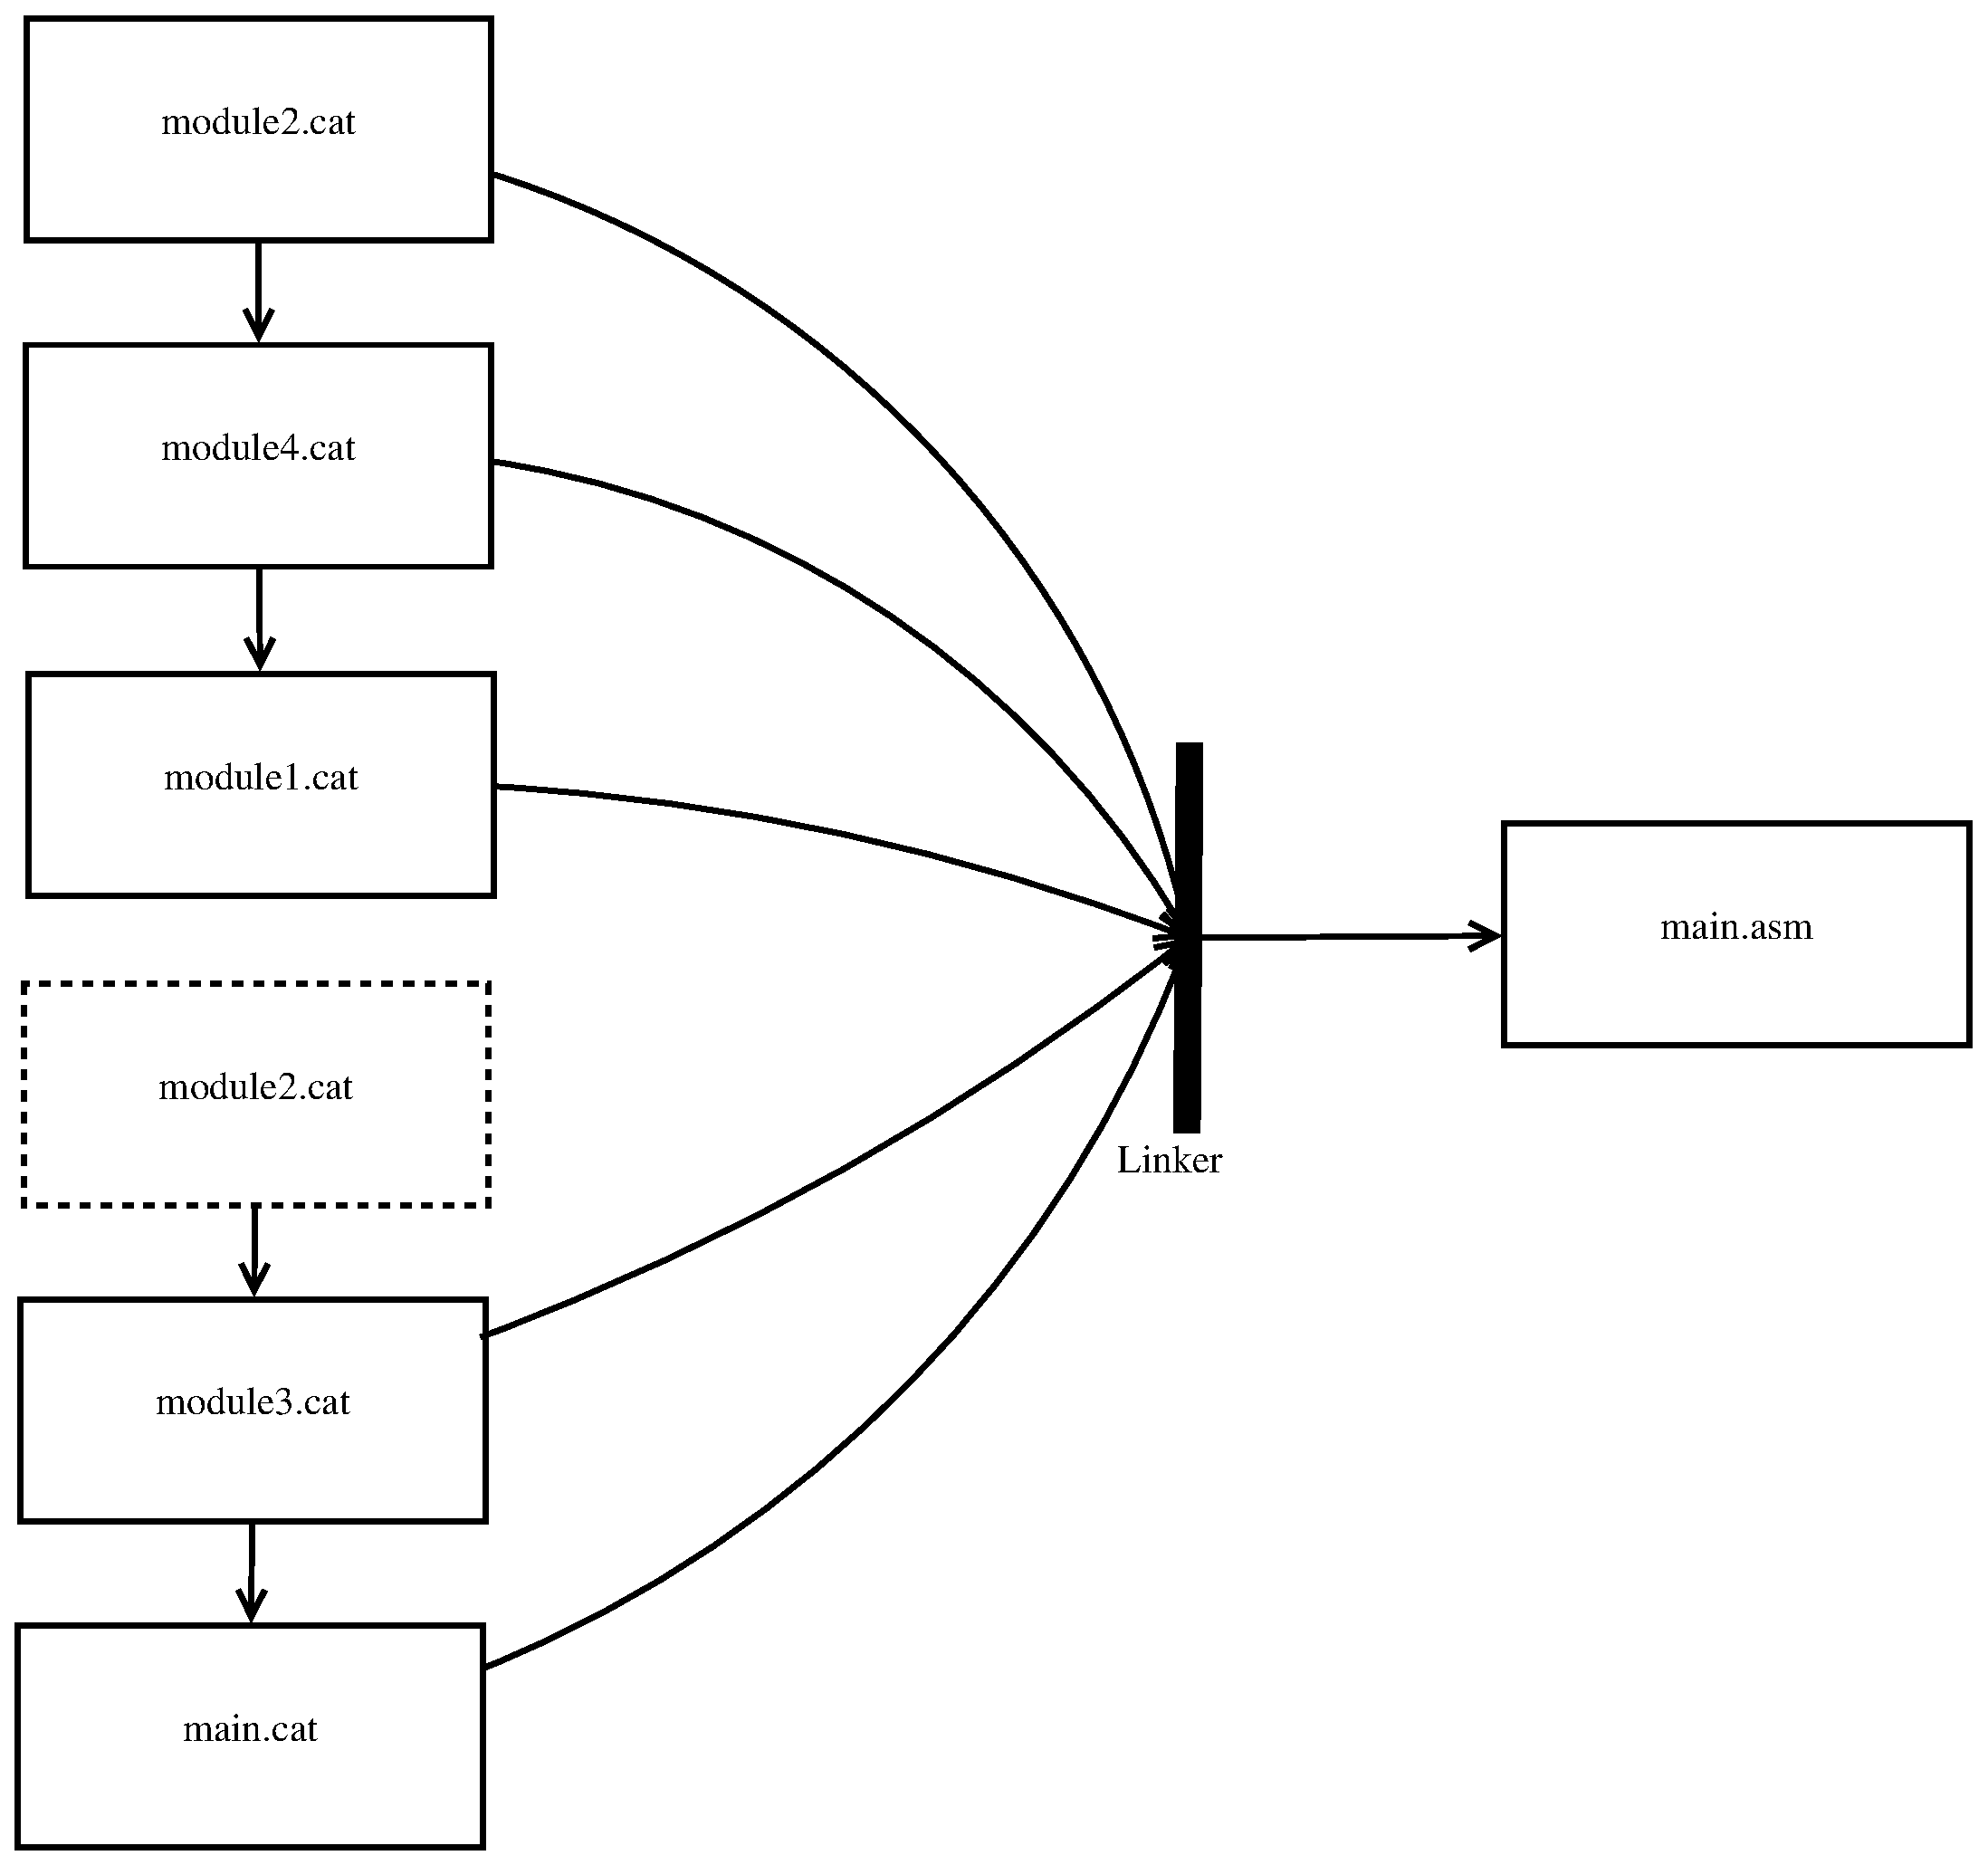
\includegraphics[width=\textwidth]{img/linking}
  \caption{The Linking Process}
  \label{fig:link}
\end{figure}

%%%%%%%%%%%%%%%%%%%%%%%%%%%%%%%%%%%%%%%%%%%%%%%%%%%%
%%%%%%%%%%%%%%%%%%%% SECTION %%%%%%%%%%%%%%%%%%%%%%%
%%%%%%%%%%%%%%%%%%%%%%%%%%%%%%%%%%%%%%%%%%%%%%%%%%%%
\section{Testing and Execution}

%%%%%%%%%%%%%%%%%%%%%%%%%%%%%%%%%%%%%%%%%%%%%%%%%%%%
%%%%%%%%%%%%%%%%%%%% SECTION %%%%%%%%%%%%%%%%%%%%%%%
%%%%%%%%%%%%%%%%%%%%%%%%%%%%%%%%%%%%%%%%%%%%%%%%%%%%
%\section{Conclusion}


\bibliographystyle{plain}
\bibliography{catpiler_doc}

\end{document}
